\begin{figure}[t]
    \centering
    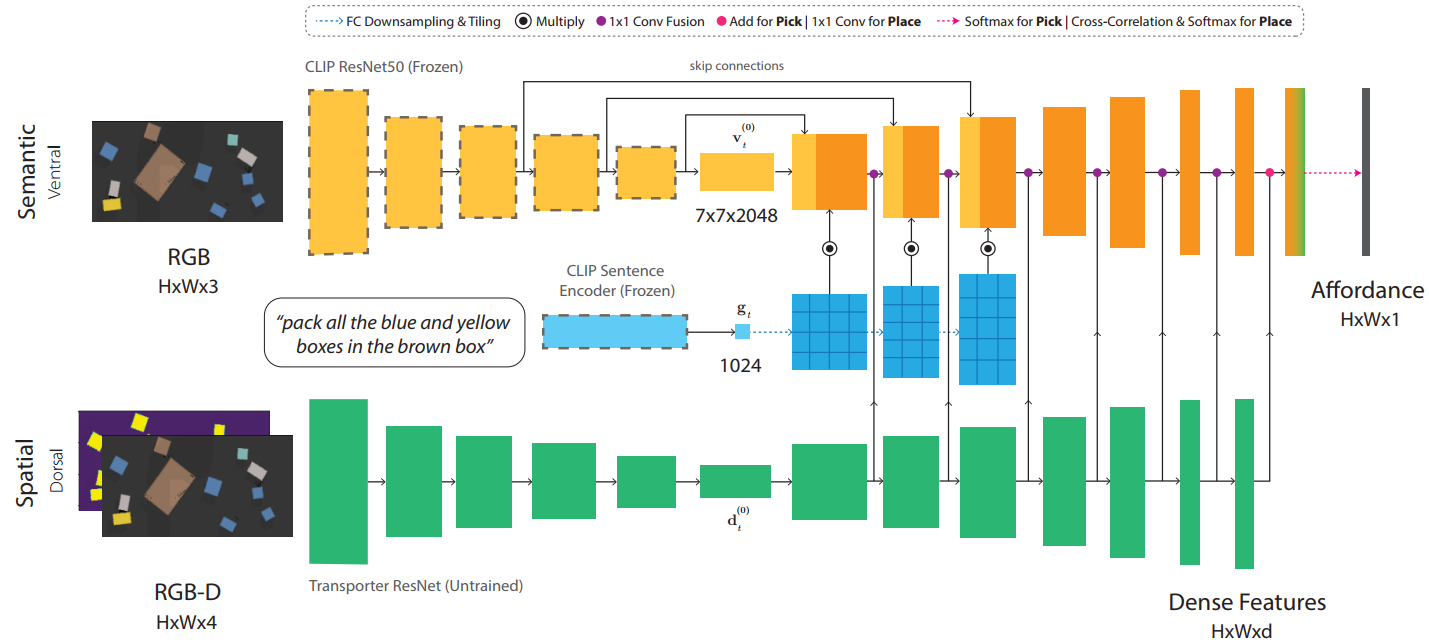
\includegraphics[width=\textwidth]{figures/images/clip_port/architecture.png}
    \caption{The Dual Stream architecture proposed in \cite{shridhar2022cliport} consists of two parallel streams: a semantic stream and a spatial stream. The semantic stream utilizes a frozen CLIP ResNet50 to encode the RGB input, with the decoder layers conditioned by tiled language features from the CLIP sentence encoder. Meanwhile, the spatial stream encodes the RGB-D input, and its decoder layers are laterally fused with those of the semantic stream. The final output is a map of dense pixelwise features, which is used to predict pick or place affordances.}
    \label{fig:clip_port_architecture}
\end{figure}

\begin{figure}[t]
    \centering
    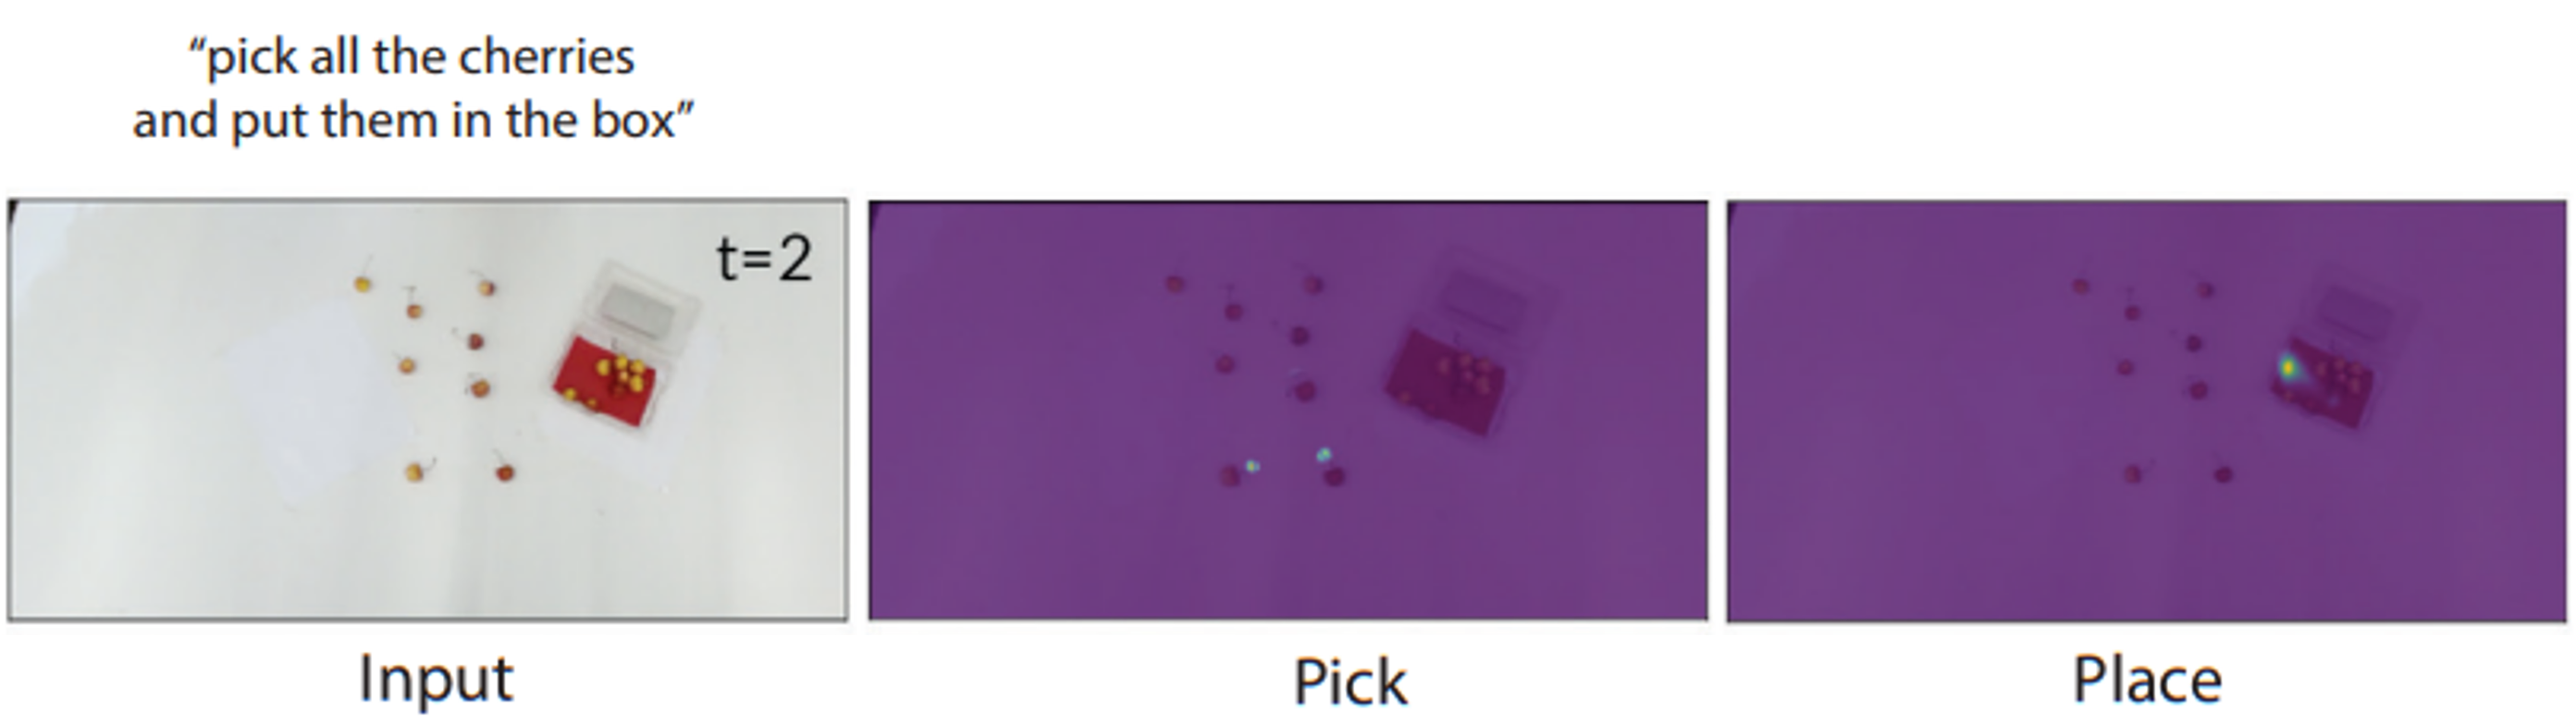
\includegraphics[width=0.8\textwidth]{figures/images/clip_port/affordance_map.png}
    \caption{Example of affordance map. (Left) The top-view input image. (Center) The affordance map for the pick-operation, since the task is to grab cherries the map highlights the two pickable cherries. (Right) The affordance map for the place operation.}
    \label{fig:clip_port_affordance}
\end{figure}